\documentclass{extbook}
\usepackage[papersize={8.5in,11in},top=1in,bottom=1in]{geometry}
\RequirePackage{fix-cm}
\usepackage[T1]{fontenc}
\usepackage{lmodern}
\usepackage{fullpage}
\usepackage{titlesec}
\usepackage{parskip}
\usepackage{float}
\usepackage{url}
\usepackage{hyperref}
\usepackage{graphicx}
\usepackage{tcolorbox}
\usepackage{tabularx}
\usepackage{xcolor}
\usepackage{titlesec}
\usepackage{amsmath}
\usepackage{tcolorbox}
\usepackage{tabularx}

\renewcommand{\contentsname}{Contenido}
\renewcommand{\figurename}{Figura}
\renewcommand{\tablename}{Tabla}
\renewcommand{\listtablename}{Lista de tablas}
\renewcommand{\listfigurename}{Lista de figuras}
\usepackage[fontsize=13.5pt]{fontsize}
\setlength{\parindent}{0pt}

\titleformat{\chapter}[display]
  {\bfseries\huge} % Estilo del título
  {\hfill\Large} % Alineación a la derecha
  {3ex} % Espaciado entre el número del capítulo y el título
  {\vspace{-5cm}\titlerule\vspace{1.5ex}\hfill} % Regla arriba y alineación del título a la derecha
  [\vspace{1ex}\titlerule] % Regla debajo del título


  \makeatletter
  \patchcmd{\chapter}
    {\if@openright\cleardoublepage\else\clearpage\fi}
    {\clearpage}
    {}{}
  \makeatother

  \definecolor{codegreen}{rgb}{0,0.6,0}
  \definecolor{codegray}{rgb}{0.5,0.5,0.5}
  \definecolor{codepurple}{rgb}{0.58,0,0.82}
  \definecolor{backcolour}{rgb}{0.95,0.95,0.92}

\begin{document}
\begin{titlepage}
  \begin{center}
      {\huge \textbf{Universidad Tecnológica de Panamá}}\\
      \vspace{3mm}
      {\Large \textbf{Centro Regional De Veraguas}}

      \begin{figure}[H]
          \centering
          
\includegraphics[scale = 0.07]{Imagenes/utp/utp.png}
          
\includegraphics[scale = 0.58]{Imagenes/utp/fisc.png}
      \end{figure}
      {\Large \textbf{Facultad de Ingeniería de Sistemas Computacionales}}\\
      \vspace{5mm}
      
      {\Large \textbf{Curso: Circuitos Lógicos}}\medskip
      
      {\Large \textbf{Profesor: Abel Rodríguez}}

      \rule{\linewidth}{0.75mm}\\
          {\Large \textsc{Informe de Laboratorio 5}} 
      \rule{\linewidth}{0.75mm}\medskip

      {\Large \textbf{Estudiantes}}\\
      \vspace{5mm}
      {\Large \textbf{Priscila Ortega, Elbin Puga, Arland Barrera, Steven Espinosa}}
      \vfill
      {\Huge \textbf{2024}}
  \end{center}
\end{titlepage}
\tableofcontents
\listoffigures
%\listoftables %para lista de tablas
\chapter{Marco Teórico}
\textbf{Arduino}

Arduino es una plataforma de hardware libre basada en una sencilla placa con un microcontrolador que se puede programar mediante el lenguaje de programación Arduino, una variante simplificada de C/C++. Es ideal para prototipos electrónicos y proyectos educativos, ya que facilita la integración de componentes electrónicos como sensores, actuadores y dispositivos de comunicación. Las placas Arduino pueden interactuar con el entorno a través de pines de entrada y salida digitales o analógicos, que permiten recibir señales y controlar dispositivos conectados.

En este contexto, se utilizan varios periféricos que pueden ser controlados desde el Arduino, como LEDs, buzzers (activos y pasivos), y otros elementos electrónicos. Su fácil manejo y flexibilidad convierten a Arduino en una herramienta potente tanto para principiantes como para ingenieros avanzados que desarrollan prototipos o aplicaciones en áreas como domótica, robótica y el Internet de las Cosas (IoT).

\textbf{Buzzers Activos y Pasivos}

Los buzzers son dispositivos piezoeléctricos que generan sonido. Existen dos tipos principales de buzzers utilizados en proyectos de Arduino: los \emph{\textbf{activos}} y los \emph{\textbf{pasivos}}.

\begin{itemize}
  \item \textbf{Buzzer Activo:} Un buzzer activo contiene un oscilador interno que genera el sonido. Solo necesita una señal de encendido/apagado desde el Arduino para funcionar, lo que simplifica su uso, ya que no requiere una señal de frecuencia de entrada. Esto lo hace ideal para aplicaciones donde se necesita simplemente activar una alerta sonora sin generar una melodía específica o controlar la frecuencia de sonido.
  \item \textbf{Buzzer Pasivo:} A diferencia del activo, el buzzer pasivo no tiene oscilador interno, por lo que necesita una señal de frecuencia externa para generar sonido. Este tipo de buzzer ofrece mayor versatilidad, ya que permite generar tonos específicos, melodías o variaciones de frecuencia, lo cual es útil en proyectos más complejos como la generación de alarmas con variación de tono o la reproducción de pequeñas melodías. Para utilizar un buzzer pasivo con Arduino, se utiliza la función \emph{tone()}, que permite generar una señal de frecuencia variable para controlar el sonido.
\end{itemize}

\textbf{LEDs (Diodos Emisores de Luz)}

Los \textbf{LEDs} son dispositivos semiconductores que emiten luz cuando son atravesados por una corriente eléctrica. Son ampliamente utilizados en proyectos de electrónica debido a su eficiencia energética, tamaño compacto, durabilidad y bajo costo. Los LEDs pueden emitir luz en diferentes colores y se usan en diversas aplicaciones como indicadores, displays o iluminación.

Un LED tiene dos terminales: el \textbf{ánodo} (positivo) y el \textbf{cátodo} (negativo). Para encender un LED, se conecta el ánodo a una fuente de corriente positiva y el cátodo a tierra, asegurándose de que la corriente sea lo suficientemente baja como para no dañar el LED. Debido a la baja corriente que soportan los LEDs, es esencial protegerlos con resistencias de limitación de corriente.

\textbf{Resistencias de Protección}

Las \textbf{resistencias} son componentes electrónicos que limitan el paso de la corriente en un circuito. En el caso de los LEDs, una resistencia de protección es crucial para evitar que el LED se queme por exceso de corriente. La cantidad de corriente que puede soportar un LED es limitada, generalmente unos 20 mA, y si se le aplica una corriente mayor, el componente puede dañarse.

Para calcular el valor de la resistencia necesaria, se utiliza la \textbf{Ley de Ohm:}

\begin{equation*}
  R = \frac{V_f - V_{LED}}{I_{LED}}
\end{equation*}

Donde:

\begin{itemize}
  \item \textbf{$R$} es el valor de la resistencia en $\Omega$ (ohmios).
  \item \textbf{$V_f$} es el voltaje de la fuente (por ejemplo, 5V en el caso de Arduino).
  \item \textbf{$V_{LED}$} es el voltaje de funcionamiento del LED (generalmente entre 1.8 y 3.3V, dependiendo del color).
  \item \textbf{$I_{LED}$} es la corriente que debe pasar por el LED (típicamente 20 mA o 0.02 A).
\end{itemize}

Una resistencia comúnmente usada para proteger LEDs es de \textbf{220 $\Omega$}, lo cual es adecuado para la mayoría de los proyectos educativos con Arduino.

\textbf{Sensores y Pines de Entrada y Salida}

En proyectos de Arduino, los sensores permiten recoger datos del entorno, como temperatura, luz o distancia. Los pines \textbf{digitales} de entrada y salida (I/O) permiten leer señales binarias (alto o bajo, 1 o 0), mientras que los pines \textbf{analógicos} permiten leer valores continuos, como la salida de un sensor de luz (LDR) o un potenciómetro.

Los pines PWM (Pulse Width Modulation) son de gran utilidad cuando se necesita simular una señal analógica. Aunque Arduino tiene pines digitales que solo pueden estar en alto (5V) o bajo (0V), mediante PWM se puede generar una señal que simula voltajes intermedios. Este principio es usado, por ejemplo, para controlar la intensidad de un LED o variar el tono de un buzzer pasivo.

\textbf{Función de Tono y Control de Sonido}

La función \emph{\textbf{tone()}} de Arduino es fundamental cuando se trabaja con buzzers pasivos. Permite generar señales de frecuencia variable que controlan el sonido emitido por el buzzer. El uso de esta función es esencial para desarrollar aplicaciones de alerta sonora o para generar melodías.
\chapter{Introducción}
El presente informe de laboratorio tiene como objetivo explorar el uso de la plataforma Arduino para la construcción y programación de circuitos electrónicos. En particular, se desarrollan una serie de ejercicios prácticos que incluyen el uso de buzzer piezoeléctrico, LEDs y resistencias, aplicando el conocimiento de programación y electrónica básica. El propósito es fomentar la comprensión del funcionamiento de los circuitos lógicos y cómo interactúan con el entorno a través de señales digitales y analógicas.

Los experimentos abarcan desde el encendido de LEDs hasta la generación de tonos con un buzzer, permitiendo a los estudiantes familiarizarse con la programación de Arduino y el montaje de circuitos sencillos. Se busca que los participantes dominen la manipulación de los componentes, el análisis de circuitos, y la interacción con el software de Arduino para programar comportamientos predefinidos.
\chapter{Cuerpo de Trabajo}
\section{Objetivos Generales}
Manipular adecuadamente la placa de arduino para completar los circuitos propuestos y posteriormente, comprender las conexiones de la placa arduino con el fin de indagar que funcionamiento tiene en la aplicación a los circuitos.
\section{Objetivos Específicos}
\begin{itemize}
  \item Entender el código de programación de la placa arduino.
  \item Entender el funcionamiento de los circuitos desarrollados.
  \item Comprender el funcionamiento del piezo (buzzer) y como impacta al funcionamiento del circuito.
\end{itemize}
\section{Materiales}
\begin{figure}[H]
  \centering
  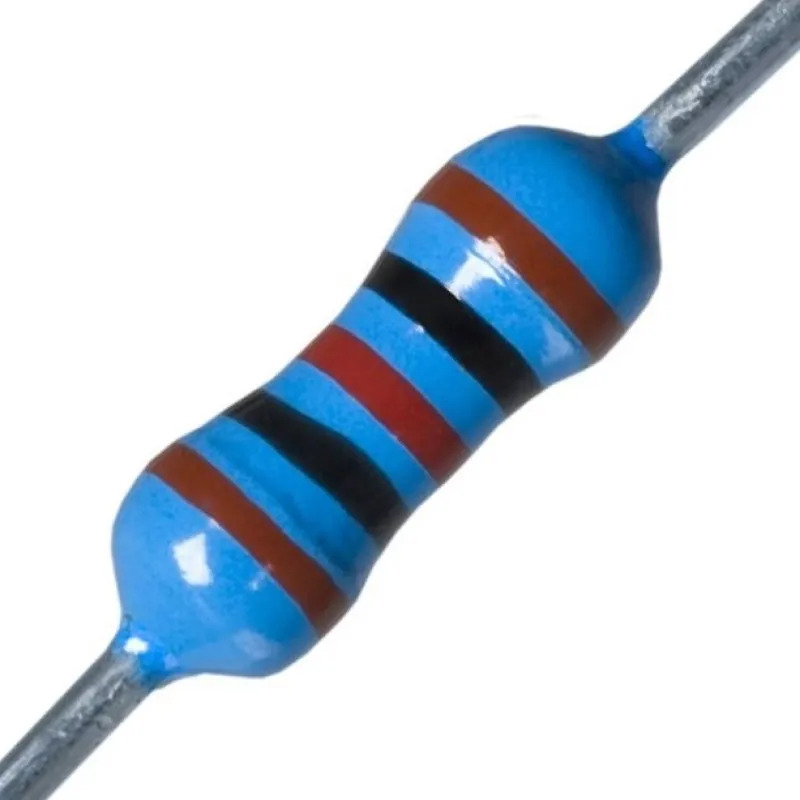
\includegraphics[scale = 0.1]{Imagenes/materiales/resistor_10k.jpg}
  \caption{Resistor de $10$ $k\Omega$}
\end{figure}

\begin{figure}[H]
  \centering
  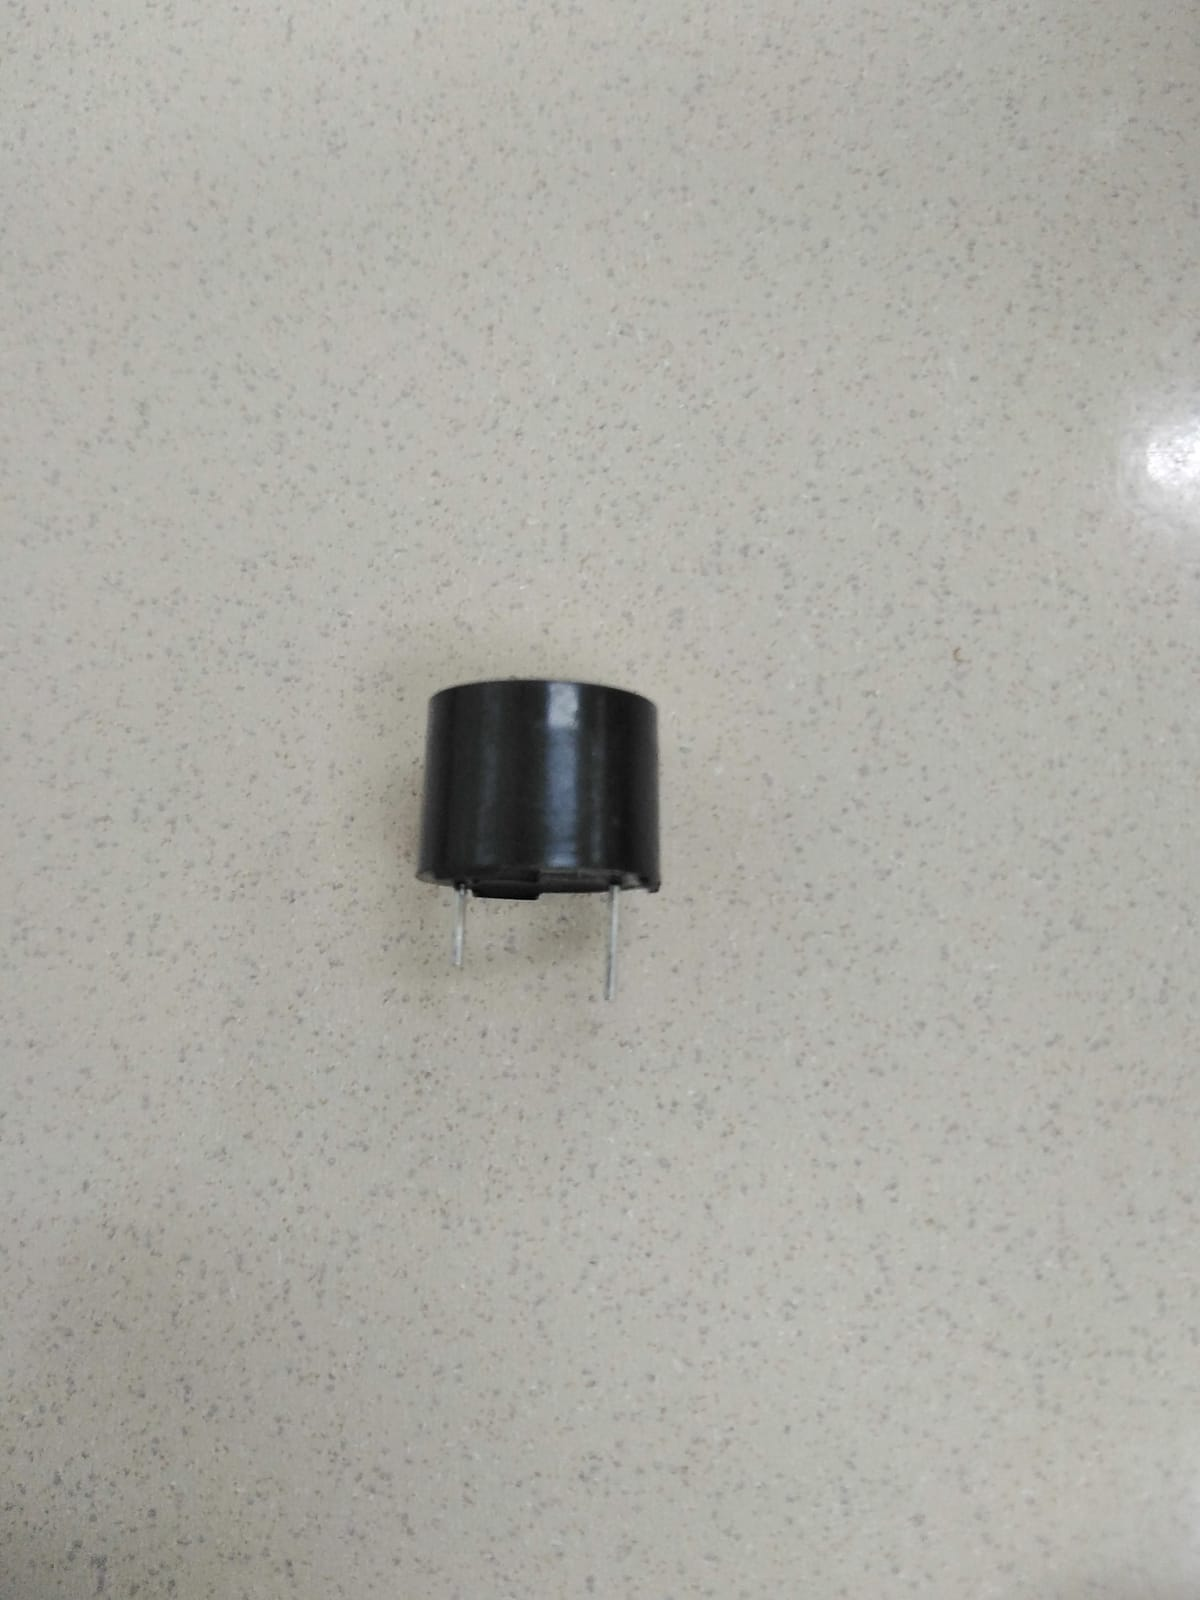
\includegraphics[scale = 0.1]{Imagenes/materiales/buzzer_activo.jpg}
  \caption{Buzzer activo}
\end{figure}
\chapter{Desarrollo}
\section{Circuitos Propuestos}
\begin{figure}[H]
  \centering
  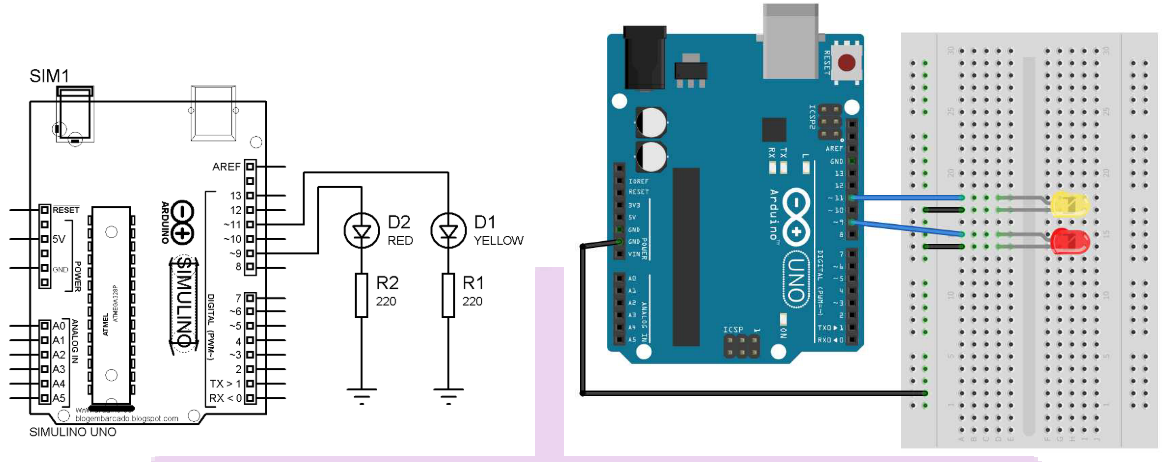
\includegraphics[scale = 0.5]{Imagenes/circPropuestos/cp_9.png}
  \caption{Circuito propuesto 9}
\end{figure}

\begin{figure}[H]
  \centering
  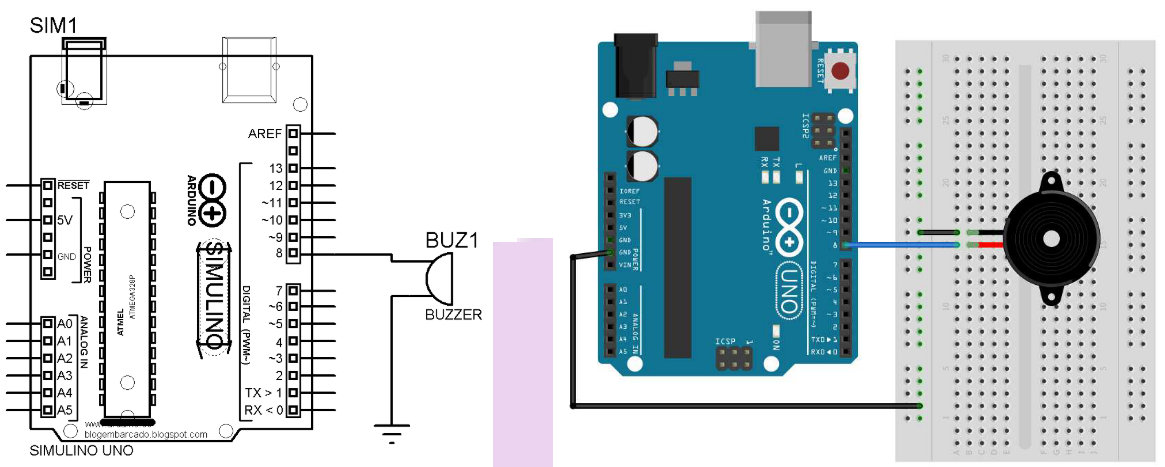
\includegraphics[scale = 0.5]{Imagenes/circPropuestos/cp_10.png}
  \caption{Circuito propuesto 10}
\end{figure}

\begin{figure}[H]
  \centering
  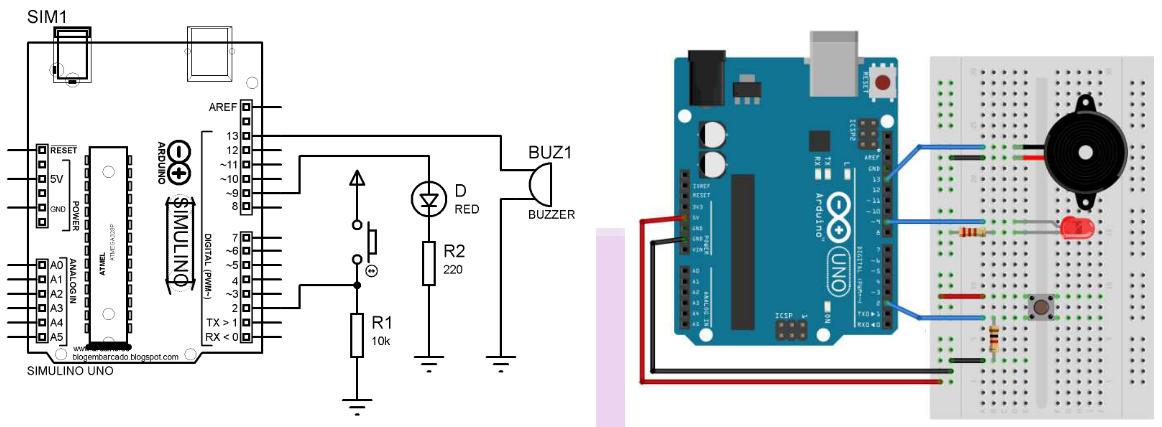
\includegraphics[scale = 0.5]{Imagenes/circPropuestos/cp_11.png}
  \caption{Circuito propuesto 11}
\end{figure}
\section{Circuitos Desarrollados}
\begin{figure}[H]
  \centering
  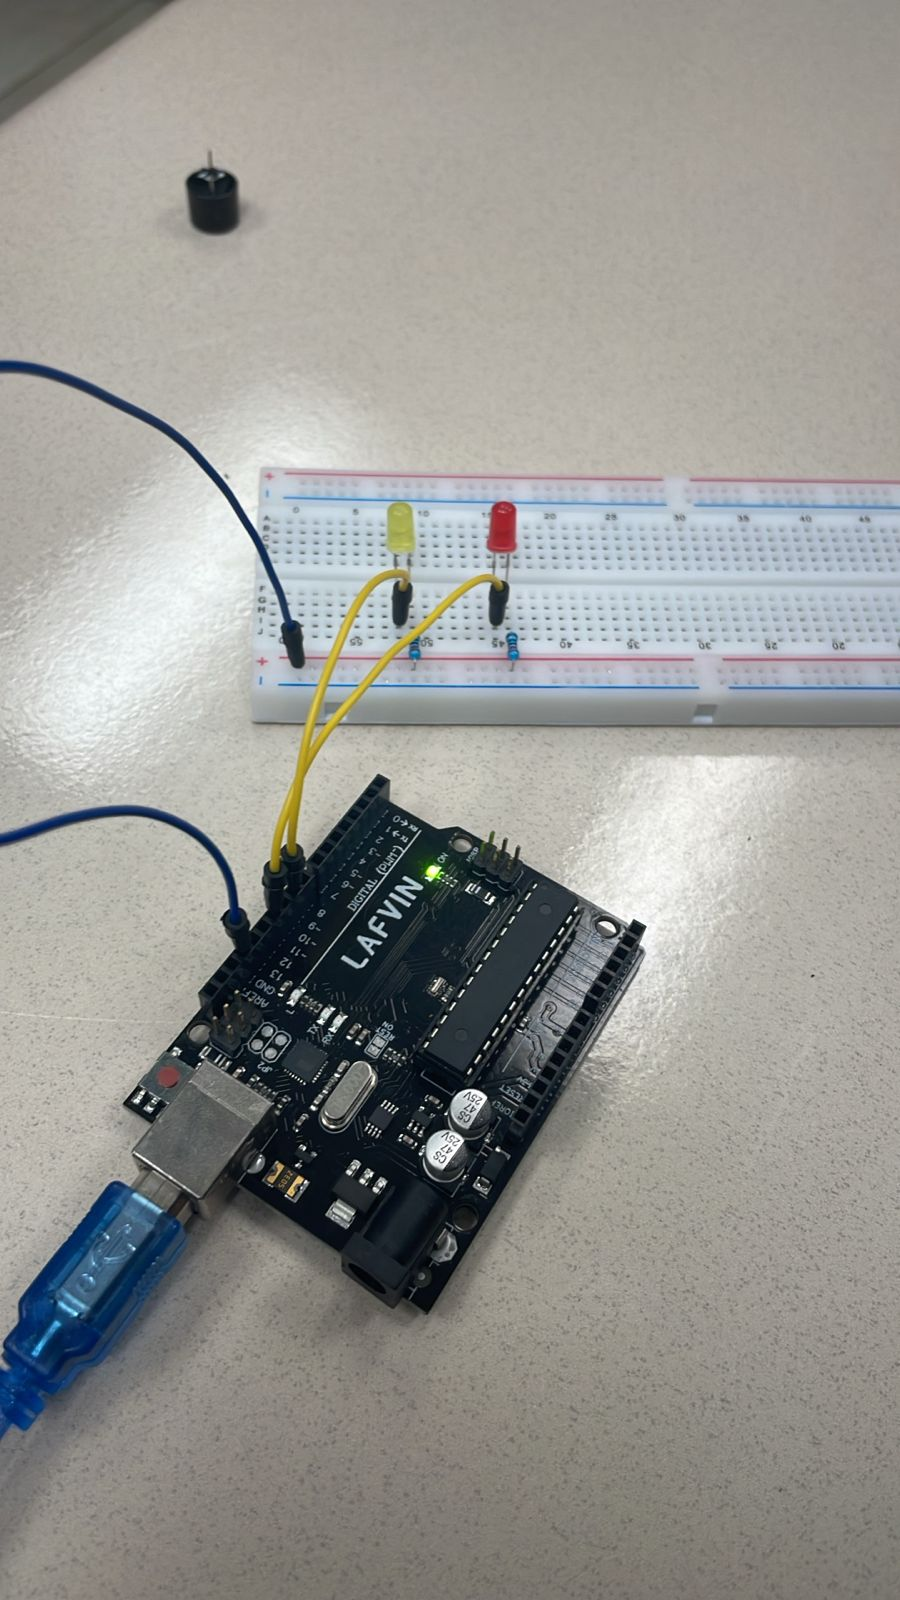
\includegraphics[scale = 0.3]{Imagenes/circDesarrollados/cd_9_circuito.jpg}
  \caption{Circuito 9 armado}
\end{figure}

\begin{figure}[H]
  \centering
  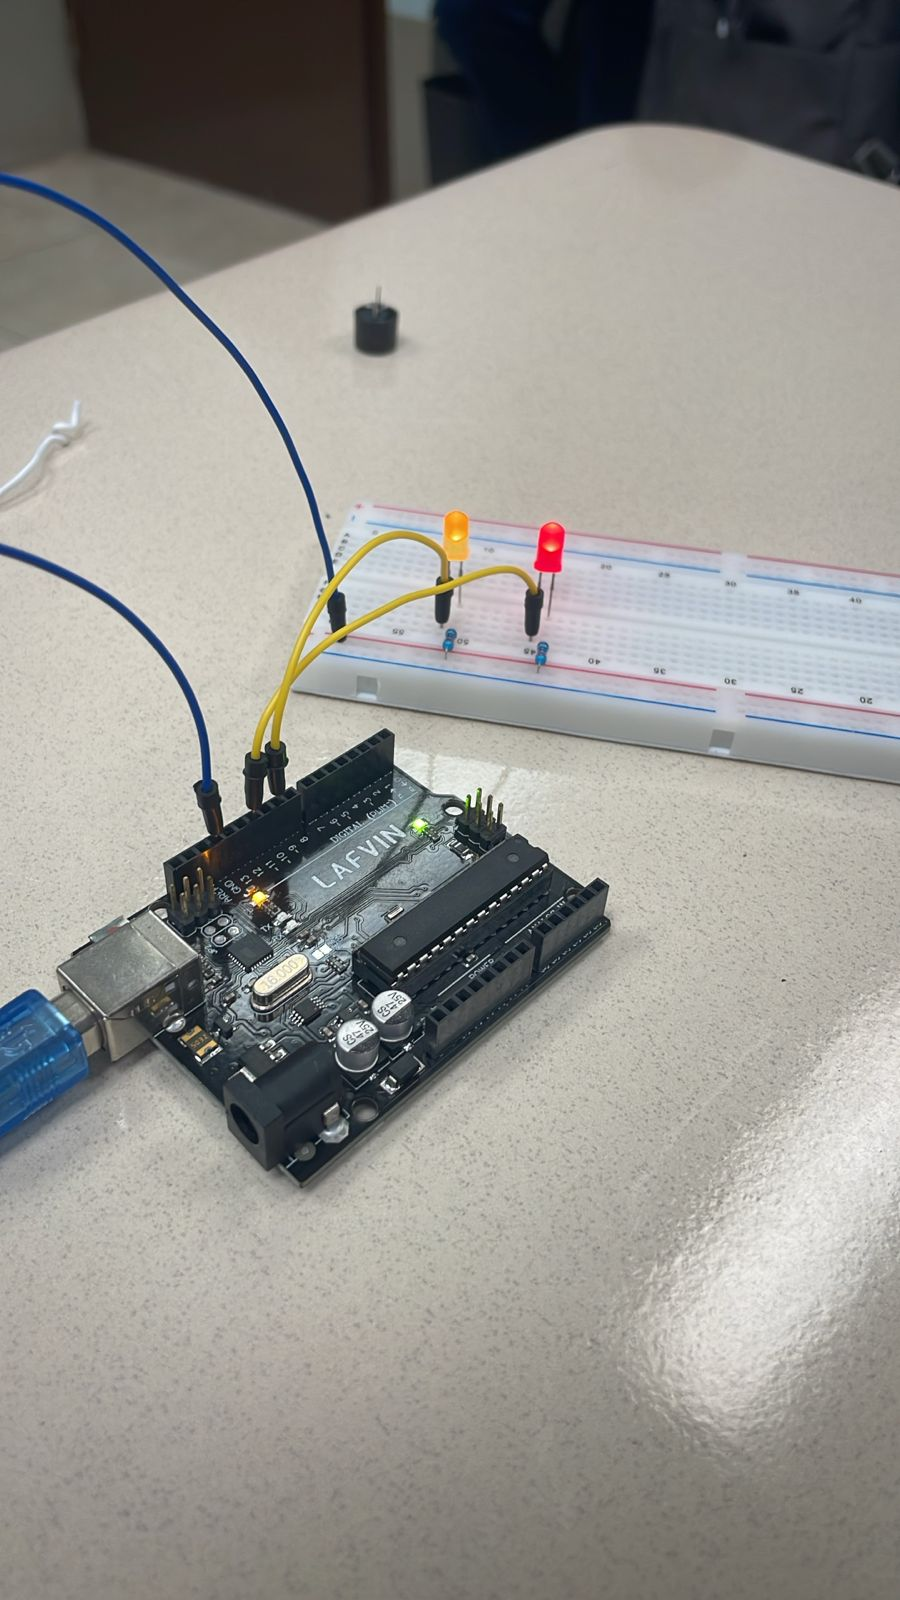
\includegraphics[scale = 0.3]{Imagenes/circDesarrollados/cd_9_ejecucion.jpg}
  \caption{Circuito 9 ejecución}
\end{figure}

\begin{figure}[H]
  \centering
  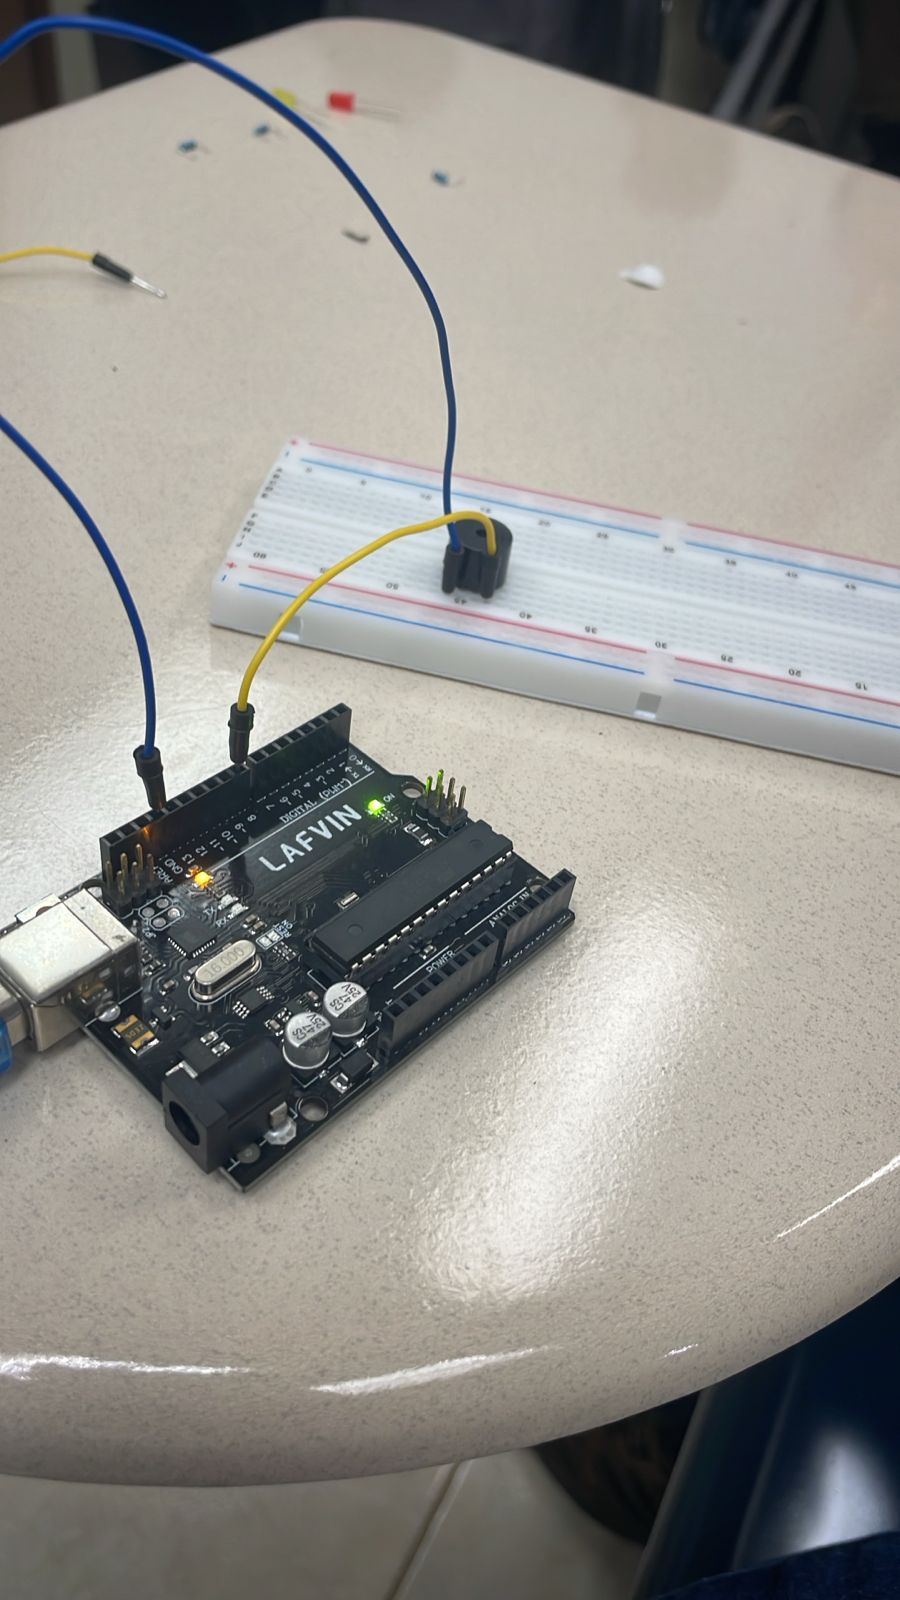
\includegraphics[scale = 0.3]{Imagenes/circDesarrollados/cd_10_circuito-ejecucion.jpg}
  \caption{Circuito 10 armado}
\end{figure}

\begin{figure}[H]
  \centering
  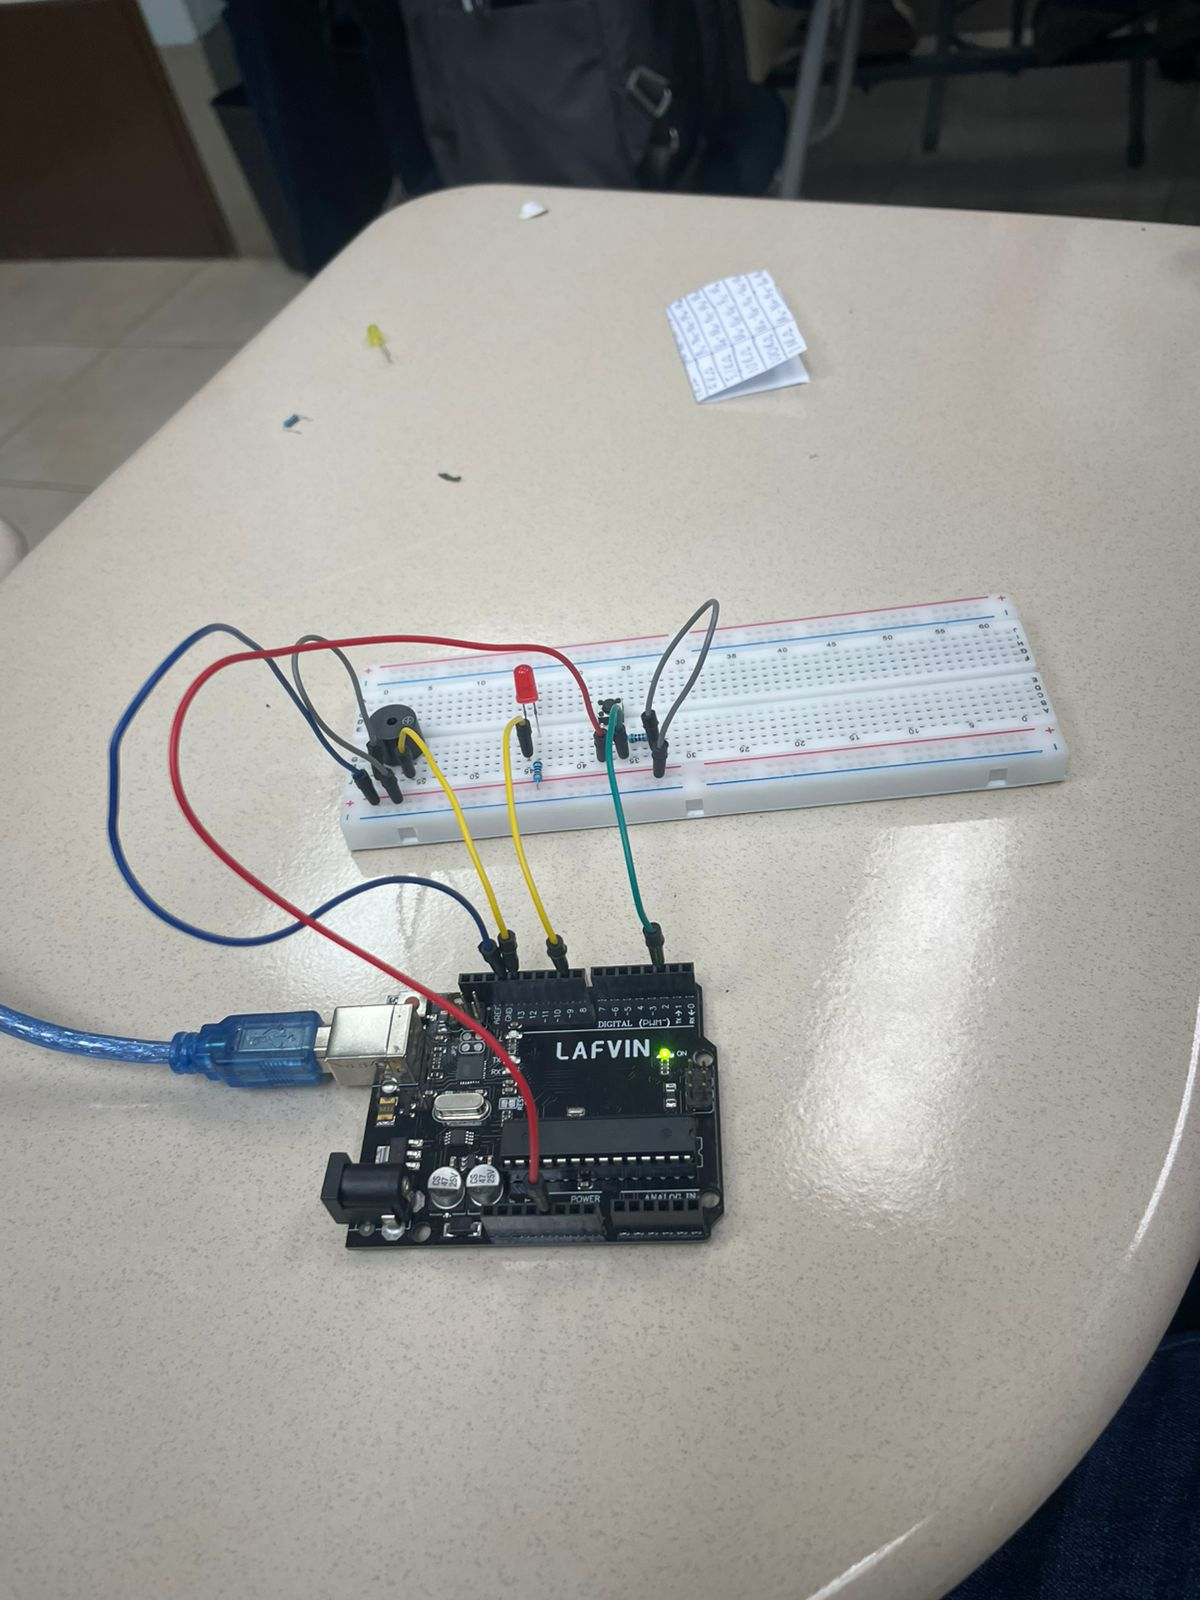
\includegraphics[scale = 0.3]{Imagenes/circDesarrollados/cd_11_circuito.jpg}
  \caption{Circuito 11 armado}
\end{figure}

\begin{figure}[H]
  \centering
  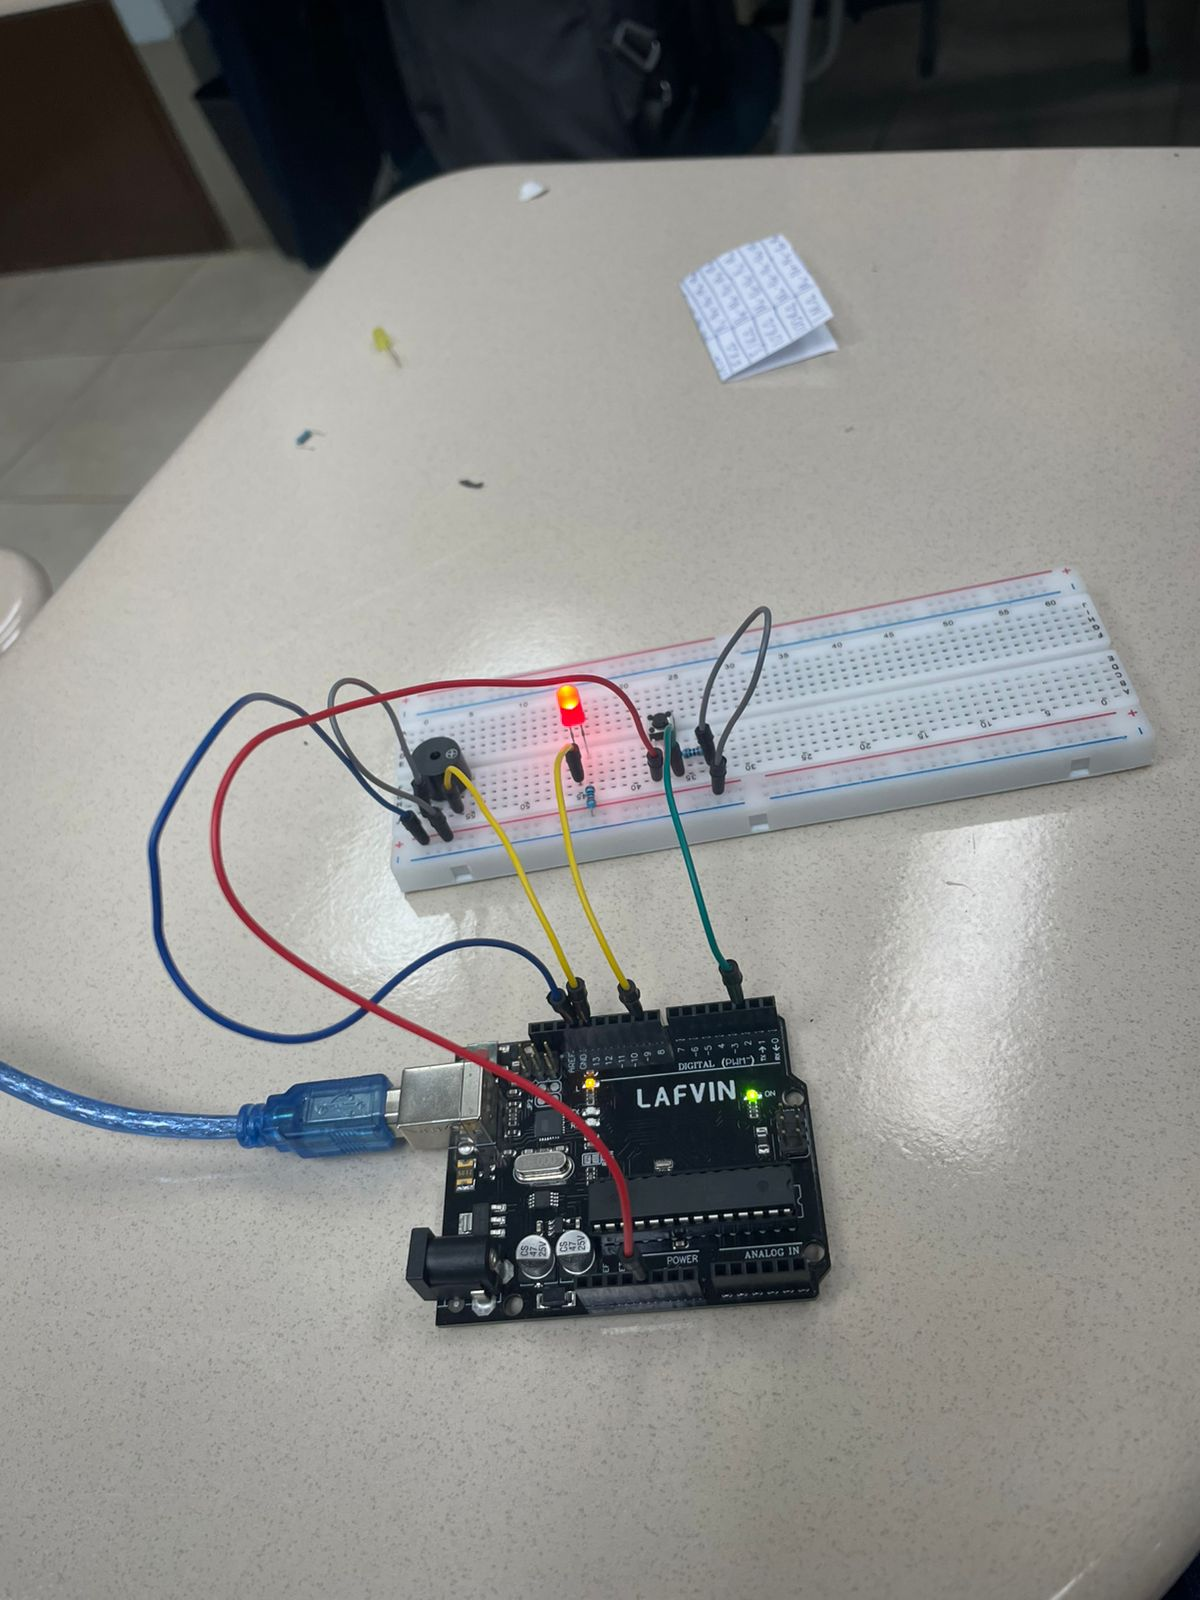
\includegraphics[scale = 0.3]{Imagenes/circDesarrollados/cd_11_ejecucion.jpg}
  \caption{Circuito 11 ejecución}
\end{figure}
\chapter{Cuestionario}
\section{Circuito 9}
¿Cómo modificarías el sketch para poder visualizar también por el serial los dos números ale torios generados en cada loop?

\emph{Código 9 Listings}

\textbf{Cambios principales:}
\begin{enumerate}
  \item \emph{Serial.begin(9600)}: Inicializa la comunicación serial a 9600 baudios.
  \item \emph{Serial.print()} y \emph{Serial.println()}: Muestra los valores aleatorios generados para los LEDs en el monitor serial.
\end{enumerate}
\section{Circuito 10}
¿Cómo harías para que el piezo tocara alguna melodía?

\emph{Código 10 Listings}

\textbf{Cambios principales:}
\begin{enumerate}
  \item Arrays \emph{melody[]} y \emph{noteDurations[]}: El array \emph{melody[]} contiene las frecuencias de las notas (en Hertz), y el array \emph{noteDurations[]} especifica la duración relativa de cada nota.
  \item \emph{noteDuration = 1000 / noteDurations[i]}: Calcula la duración real de cada nota en milisegundos.
  \item \emph{tone(buzzer, melody[i], noteDuration)}: Reproduce la nota correspondiente del array \emph{melody[]} con la duración calculada.
  \item \emph{delay(noteDuration * 1.30)}: Añade una ligera pausa entre las notas para que suene de manera más natural.
\end{enumerate}
\section{Circuito 11}
¿Cómo harías para que en vez de 10 ciclos fuesen 15 ciclos y cada ciclo durase 20 ms menos?

\emph{Código 11 Listings}

\textbf{Cambios principales:}
\begin{enumerate}
  \item Ciclos en el \emph{for}: Cambiar el límite de \emph{i <= 10} a \emph{i <= 15} para hacer 15 ciclos.
  \item Duración de los ciclos: Reducir los \emph{delay(100)} a \emph{delay(80)} para que cada ciclo sea 20 ms más corto ($100 ms - 20 ms = 80 ms$).
\end{enumerate}
\chapter{Conclusiones}
A lo largo de la práctica de laboratorio, se logró un dominio fundamental en el uso de Arduino para controlar dispositivos electrónicos, así como en la programación de su microcontrolador. Se pudo evidenciar que la plataforma es accesible tanto para principiantes como para proyectos más avanzados, debido a su flexibilidad y a la vasta cantidad de recursos disponibles.

El uso de circuitos sencillos con LEDs y buzzers permitió a los estudiantes comprender el funcionamiento básico de los componentes electrónicos, así como su programación. Asimismo, la interacción con la comunicación serie facilitó el monitoreo de datos en tiempo real, una habilidad crucial para el desarrollo de proyectos electrónicos más complejos.

Finalmente, se destaca la importancia de la correcta interpretación de los esquemas eléctricos y la adecuada disposición de los componentes en un protoboard, lo que facilita la comprensión teórica y la práctica de conceptos de electrónica y programación.
\chapter{Referencias}
Arduino R3. (2024). *Arduino product reference manual. \url{https://docs.arduino.cc/}

OIKOS MATEMATIKÓN PRÁCTICAS DE ARDUINO. Proporcionado por el profesor Abel Rodríguez
\chapter{Anexos}
\section{Datos de los materiales usados}
\begin{enumerate}
  \item \textbf{Circuito Integrado (IC) de Arduino}
  \begin{itemize}
    \item \textbf{Modelo:} LAFVIN Arduino R3
    \item \textbf{Microcontrolador:} ATmega328P (similar al Arduino UNO)
    \item \textbf{Arquitectura:} 8 bits
    \item \textbf{Memoria Flash:} 32 KB 
    \item \textbf{RAM:} 2 KB 
    \item \textbf{EEPROM:} 1 KB 
    \item \textbf{Pines Digitales I/O:} 14 
    \item \textbf{Pines Analógicos I/O:} 6
    \item \textbf{PWM:} 6 
    \item \textbf{Timers:} 3 
    \item \textbf{UARTs:} 1 
    \item \textbf{SPI:} 1
    \item \textbf{12C:} 1
  \end{itemize}
  \item \textbf{LEDs (Diodos Emisores de Luz)}
  \begin{itemize}
    \item \textbf{Tipo:} LED estándar de 5 mm
    \item \textbf{Color:} Rojo y amarillo
    \item \textbf{Tensión de Funcionamiento (VF):} 2-3.5V
    \item \textbf{Corriente de Funcionamiento:} 20 mA
  \end{itemize}
  \item \textbf{Jumpers (Cables de Conexión)}
  \begin{itemize}
    \item \textbf{Tipo:} Cables de conexión macho-macho, macho-hembra, hembra-hembra
    \item \textbf{Longitud:} 15 cm a 30 cm
  \end{itemize}
  \item \textbf{Pulsadores (Botones)}
  \begin{itemize}
    \item \textbf{Tipo:} Pulsador momentáneo
    \item \textbf{Número de Pines:} 4
    \item \textbf{Tensión Máxima:} 12 V
    \item \textbf{Corriente Máxima:} 0.5 A
    \item \textbf{Dimensiones:} Aproximadamente 6x6 mm
  \end{itemize}
  \item \textbf{Protoboard (Breadboard)}
  \begin{itemize}
    \item \textbf{Tipo:} Protoboard estándar
    \item \textbf{Dimensiones:} Comúnmente 830 puntos
  \end{itemize}
  \item \textbf{Resistor de 220 $\Omega$ (Ohmios) a 1/4 W}
  \begin{itemize}
    \item \textbf{Valor:} 220 $\Omega$
    \item \textbf{Tolerancia:} ±1
    \item \textbf{Potencia Nominal:} 12 V
  \end{itemize}
  \item \textbf{Resistor de 10 $k\Omega$ (Ohmios) a 1/4 W}
  \begin{itemize}
    \item \textbf{Valor:} 10 $k\Omega$
    \item \textbf{Tolerancia:} ±1
    \item \textbf{Potencia Nominal:} 12 V
  \end{itemize}
  \item \textbf{Piezo (Buzzer) Activo}
  \begin{itemize}
    \item \textbf{Voltaje Nomianl:} 5 V
    \item \textbf{Voltaje de funcionamiento:} 4 - 8 V
    \item \textbf{Corriente nominal máxima:} <=32 mA
    \item \textbf{Frecuencia resonante:} 2300 ±300 Hz
    \item \textbf{Temperatura de funcionamiento:} -20°C to 45°C
    \item \textbf{Dimensiones (sin pines)}
    \begin{itemize}
      \item \textbf{Altura:} 9.16 mm (0.36")
      \item \textbf{Diámetro:} 11.78 mm (0.46")
      \item \textbf{Peso:} 1.6 g (0.057 oz)
    \end{itemize}
  \end{itemize}
\end{enumerate}
\section{Alcance de la aplicación de este laboratorio a futuro}
El laboratorio de Arduino tiene un amplio alcance para aplicaciones futuras, especialmente en el campo de la automatización, el control de sistemas y la enseñanza de electrónica básica. Los conocimientos adquiridos pueden aplicarse en áreas como la robótica, el internet de las cosas (IoT), y el desarrollo de sistemas embebidos.

A nivel educativo, este tipo de prácticas fomenta el aprendizaje activo y permite a los estudiantes aplicar sus conocimientos en la creación de prototipos reales, lo que a su vez refuerza la comprensión de los principios teóricos de la electrónica. En el ámbito profesional, las aplicaciones prácticas de Arduino permiten diseñar sistemas de control eficientes y económicos, abriendo puertas a innovaciones tecnológicas tanto en el ámbito industrial como en el doméstico.
\end{document}